\documentclass[a4paper,11pt,twoside]{article}
%\documentclass[a4paper,11pt,twoside,se]{article}

\usepackage{UmUStudentReport}
\usepackage{verbatim}   % Multi-line comments using \begin{comment}
\usepackage{courier}    % Nicer fonts are used. (not necessary)
\usepackage{pslatex}    % Also nicer fonts. (not necessary)
\usepackage[pdftex]{graphicx}   % allows including pdf figures
\usepackage{listings}
\usepackage{pgf-umlcd}
\usepackage{blindtext}
\usepackage{enumitem}
\usepackage{amsfonts}
\usepackage{mathtools}
%\usepackage{lmodern}   % Optional fonts. (not necessary)
%\usepackage{tabularx}
%\usepackage{microtype} % Provides some typographic improvements over default settings
%\usepackage{placeins}  % For aligning images with \FloatBarrier
%\usepackage{booktabs}  % For nice-looking tables
%\usepackage{titlesec}  % More granular control of sections.

% DOCUMENT INFO
% =============
\department{Department of Computing Science}
\coursename{Parallel Programming 7.5 p}
\coursecode{5DV152}
\title{Exercises, Chapter/Topic 3}
\author{Lorenz Gerber ({\tt{dv15lgr@cs.umu.se}} {\tt{lozger03@student.umu.se}})}
\date{2017-02-16}
%\revisiondate{2016-01-18}
\instructor{Lars Karlsson / Mikael Ränner}


% DOCUMENT SETTINGS
% =================
\bibliographystyle{plain}
%\bibliographystyle{ieee}
\pagestyle{fancy}
\raggedbottom
\setcounter{secnumdepth}{2}
\setcounter{tocdepth}{2}
%\graphicspath{{images/}}   %Path for images

\usepackage{float}
\floatstyle{ruled}
\newfloat{listing}{thp}{lop}
\floatname{listing}{Listing}



% DEFINES
% =======
%\newcommand{\mycommand}{<latex code>}
\DeclarePairedDelimiter{\ceil}{\lceil}{\rceil}
\DeclarePairedDelimiter{\floor}{\lfloor}{\rfloor}

% DOCUMENT
% ========
\begin{document}
\lstset{language=C}
\maketitle
\thispagestyle{empty}
\newpage
\tableofcontents
\thispagestyle{empty}
\newpage

\clearpage
\pagenumbering{arabic}

\section{Introduction}
This report is part of the mandatory coursework. It describes the solutions for several chosen exercises from the course book \cite{pacheco2011}.

\section{3.2 - Generalization of algorithm for trapezoidal rule}
Two functions to adapt the \textit{trapezoidal rule} for \verb+calc\_local\_a+ and \verb+calc\_local\_b+ were written and tested with the source code from the book (\textit{mpi\_trap.c}). The source can be found in appendix \ref{app:source32}.

\section{3.6 - Array distributions}

\subsection*{Block distribution}
Block distribution can be obtained by $b = \floor*{i \div p}$ where $b$ is the block number, $i$ the index of $n$ and $p$ is the number of processes. This solution is however not fair. An improved, fair expression can be devised using ternary operators:
\begin{equation*}
i< n\bmod p \times \ceil*{n \div p} ? \floor*{i \div \ceil*{n \div p}} : n\mod p + \floor*{(i -n\mod p \times \ceil*{n \div p}) \div \floor*{n\mod p}}
\end{equation*} 

\subsection*{Cyclic distribution}
Cyclic distribution is described by $b = i\mod p$ with $b$ as block number $i$ as index of $n$ and $p$ as number of processes. 

\subsection*{Block cyclic distribution}
Block cyclic distribution can be expressed as $b = \floor*{i \div l} mod p$ where $b$ is block index, $i$ index of $n$, $l$ block length and $p$ number of processes.

\section{3.8 - Tree-structured algorithms for scatter and gather}
The diagram for tree-structured scatter is shown in figure \ref{fig:scatter}. The arrows show the communication events which for the present case of \verb+comm_sz = 8+ and \verb+n = 16+ is 7. This is also true for the tree-structured gather shown in figure \ref{fig:gather}.
\begin{figure}
  \centering
  
\includegraphics[width=1\textwidth]{scatter.png}
  \caption{\textit{This graph shows a tree based implementation of scatter for comm\_sz = 8 and n = 16. It has 7 communication events.}}
  \label{fig:scatter}
\end{figure}
\begin{figure}

  \centering
  
\includegraphics[width=1\textwidth]{gather.png}
  \caption{\textit{This graph shows a tree based implementation of gather for comm\_sz = 8 and n = 16. It has 7 communication events.}}
  \label{fig:gather}
\end{figure}

\section{3.9 - Vector scaling and dot product}
The Source code for the vector scaling and dot product MPI program can be found in appendix \ref{app:source39}.


\section{3.11 - Prefix sums}
\subsection*{Serial Algorithm}
Assume vector $x$ of length $n$ and prefix sums vector $y$ to be calculated.
\begin{verbatim}
y_0 = x_0
for (i = 1, i < n , i++)
    y_i = y_i-1 + n_i
\end{verbatim}

\subsection*{Parallel Algorithm}
After Blelloch \cite{blelloch1990}, parallel prefix-sum, or `Sum Scan Algorithm' can be calculated in two steps, the `Up-sweep' (Reduce) and `Down-sweep'. Below, pseudo code from Valdez \cite{valdez2012} where $x$ is the input data, $n$ the size of the input and $d$ the number of processeors. If $n \neq 2^{k}$, then $n$ has to be extended with \textit{zero's}. The `Up-Sweep':
\begin{verbatim}
for d = 0 to log2(n) – 1 do 
      for all k = 0 to n – 1 by 2^(d+1) in parallel do 
           x[k +  2^(d+1) – 1] = x[k +  2^d  – 1] + x[k +  2^(d+1) – 1]
\end{verbatim}

The `Down-Sweep':
\begin{verbatim}
x[n – 1] = 0
 for d = log2(n) – 1 down to 0 do 
       for all k = 0 to n – 1 by 2^(d+1) in parallel do 
            t = x[k +  2^d  – 1]
            x[k +  2^d  – 1] = x[k +  2^(d+1) – 1]
            x[k +  2^(d+1) – 1] = t +  x[k +  2^(d+1) – 1]

\end{verbatim}

\subsection*{Minimum Communication}
An algorithm that uses for the prefix-sum of length $n = 2^k$ only $k$ communication steps can be derived from the communication model in a hypercube as shown in figure \ref{fig:hypercube}.

\begin{figure}

  \centering
    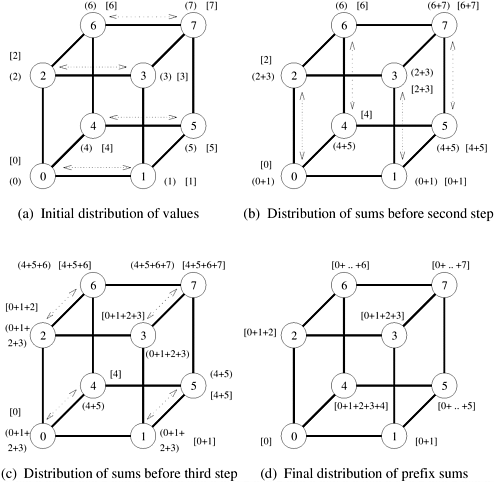
\includegraphics[width=1\textwidth]{hypercube.png}
    \caption{\textit{This figure shows the calculation of prefix sums with minimal communication phases. The figure is take from \cite[chap 4.3]{grama2003}}}
    \label{fig:hypercube}
\end{figure}

Below follows pseudo code for parallel hypercube prefix sum (from \cite{grama2003}):

\begin{verbatim}
procedure PREFIX_SUMS_HCUBE(my_id, my number, d, result) 
   begin 
      result := my_number; 
      msg := result; 
      for i := 0 to d - 1 do 
          partner := my_id XOR 2i; 
          send msg to partner; 
          receive number from partner; 
          msg := msg + number; 
          if (partner < my_id) then result := result + number; 
      endfor; 
   end PREFIX_SUMS_HCUBE
\end{verbatim}



\subsection*{MPI Program using MPI\_Scan}
A minimal working example using MPI\_Scan was implemented. The source code can be found in appendix \ref{app:source311}. An array of random numbers are generated on each proces. Then the prefix sums are collected onto process zero. The prefix sums of the arrays are collected index wise. Arrays or length n and p processes will result in a n $\times$ p prefix sum array.  


\section{3.13 - Generalization of vector scaling and dot product}
An MPI program for `Vector Scaling and Dot Product' using `MPI\_Scatterv'/`MPI\_Gatherv' was written according to the specifications. The source code can be found in appendix \ref{app:source313}.

\section{3.16 - Diagram for a butterfly implementation of allgather}
Figure \ref{fig:allgather} shows an diagram for an \textit{allgather} implementation using \textit{butterfly} communication. The exmples shows the communication steps for 8 processes and a data vector length of 16.  
\begin{figure}
  \centering
    
\includegraphics[width=1\textwidth]{allgather.png}
    \caption{\textit{This figure shows a butterfly allgather implementation for 8 cores and a vector of length 16.}}
    \label{fig:allgather}
\end{figure}



\section{3.18 - Derived data types}
Here \verb+MPI\_Type\_vector+ was used to implement a derived data type to represent a block cyclic data distribution. The current implementation assumes that the data is even divisible by blocksize $\times$ processes. This allows to use only one data type definition for the full length block cyclic structe of one process. The source code can be found in appendix \ref{app:source318}

\section{3.20 - Pack and unpack}
The MPI functions MPI\_Pack and MPI\_Unpack were used transfer complex datastructures. As example, a new \textit{Get\_input} function for the `trapezoidal sum' program was written that transfers the data from process 0 to all processes. The source code of the modified \textit{Get\_input} function can be found in appendix \ref{app:source320}.

\section{3.21 - Matrix-vector multiplication}
The `Matrix-vector multiplication' program from the course book was run on the HPC2N \textit{Abisko} cluster for benchmarking and comparison to the values in the course book. Herefore the source \textit{mpi\_mat\_vect\_time.c} provided from the coursebooks homepage was compiled with MPI-gcc compiler on the Abisko cluster. Problemsize and process number were chosen accoring to the example in the course book.

\subsection{Speed comparison}
The absolute run-times values differ significantly from the benchmarked system in the book, see \cite[p. 123]{pacheco2011} and table \ref{tab:runtimes}. The bechmarking was run on the `abisko' cluster with the setting to run one process per node. For such a small program, this was performance wise probably not the most optimal choice: It can be seen in table \ref{tab:runtimes} that all runtimes for 16 processes are longer than those for respective problem size and fewer processes. Most likely, this is due to the higher communication overhead.  
\begin{table}[]
\centering
\caption{\textit{Median runtimes for the Matrix-Vector Multiplication. The program was run on the HPC2N `abisko' cluster. Processes were assigned to individual nodes.}}
\label{tab:runtimes}
\begin{tabular}{cccccc}
\multicolumn{1}{l|}{}         & \multicolumn{5}{l|}{Order of Matrix (milliseconds)}                                                                   \\ \cline{2-6} 
\multicolumn{1}{l|}{comm\_sz} & \multicolumn{1}{c|}{1024} & \multicolumn{1}{c|}{2048} & \multicolumn{1}{c|}{4096} & \multicolumn{1}{c|}{8192} & 16384 \\
1                             & 0.01                      & 0.02                      & 0.03                      & 0.07                      & 0.14  \\
2                             & 0.01                      & 0.02                      & 0.02                      & 0.04                      & 0.08  \\
4                             & 0.01                      & 0.02                      & 0.02                      & 0.03                      & 0.04  \\
8                             & 0.02                      & 0.02                      & 0.02                      & 0.02                      & 0.03  \\
16                            & 0.03                      & 0.03                      & 0.03                      & 0.03                      & 0.05 
\end{tabular}
\end{table}


\subsection{Observed variabilities}
Variability was assessed using boxplots, see figure \ref{fig:boxplot}.
\begin{figure}
  \centering
    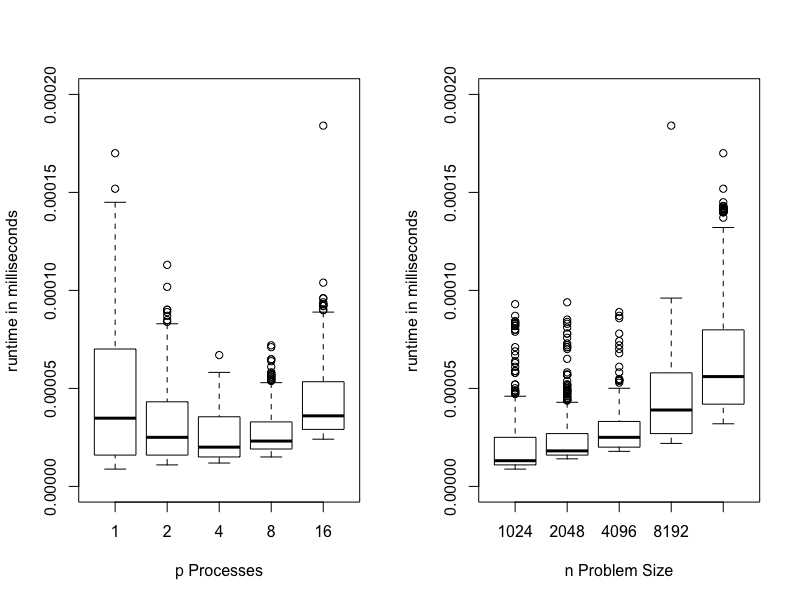
\includegraphics[width=1\textwidth]{boxplot.png}
    \caption{\textit{This figure shows boxplot of runtimes in relation to number of processes and problem size.}}
    \label{fig:boxplot}
\end{figure}



\subsection{Cluster around Minmum, mean, median}

For the clustering of minumum, mean and median, plot showing the timings normalized to their respective largest value were plotted. In each plot series, mean and median were also shown (Figure \ref{fig:spread}).

\begin{figure}
  \centering
    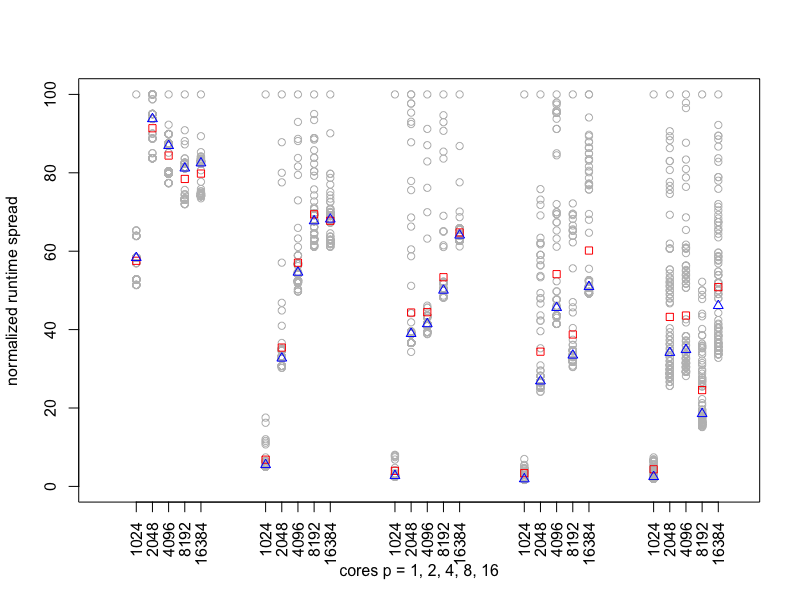
\includegraphics[width=1\textwidth]{spread.png}
    \caption{\textit{This figure shows the normalized ranges of runtimes to compare mimima, maxima, median and mean values. Mean values are marked by a red square and median values by a blue cirlce}}
    \label{fig:spread}
\end{figure}


\section{3.22 - Timing the trapezoidal rule}
The problem size should be select in a way that the runtimes occour in a regime that is measurable with the given precision of the timing functionality. Further, it is favourable to have a series of multiples i.e the double, the quadruple etc. Here it was chose to use the series 65536, 131072, 262144, 524288, 1048576 as problem size n for the number of trapezoids.

Here, the parameters for the batch runs on HPC2N's `abisko' were chose to assign one processor for each process instead of a whole node for each process. This had certainly a positive effect on lowering the communication overhead for higher number of processes. 

\begin{table}[]
\centering
\caption{\textit{This table shows the mean of the benchmarking values for the trapezoidal rule}}
\label{tab:mean_trap}
\begin{tabular}{llllll}
\multicolumn{1}{l|}{}          & \multicolumn{5}{c}{number of trapezoids}                                                                                       \\ \cline{2-6} 
\multicolumn{1}{l|}{processes} & \multicolumn{1}{l|}{65536} & \multicolumn{1}{l|}{131072} & \multicolumn{1}{l|}{262144} & \multicolumn{1}{l|}{524288} & 1048576 \\ \hline
1                              & 0.73                       & 1.36                        & 2.70                        & 5.39                        & 10.77   \\
2                              & 0.31                       & 0.62                        & 1.23                        & 2.46                        & 4.91    \\
4                              & 0.16                       & 0.33                        & 0.67                        & 1.29                        & 2.59    \\
8                              & 0.09                       & 0.17                        & 0.33                        & 0.66                        & 1.32    \\
16                             & 0.27                       & 0.10                        & 0.22                        & 0.35                        & 0.73   
\end{tabular}
\end{table}

In most cases, median (table \ref{tab:median_trap}) and mean values (\ref{tab:mean_trap}) were just a few digits apart, with the median always being the lower. However, in some cases the sensitivity of the mean towards outliers can be see. For example for the mean time of $p = 16$ ane $n = 65536$ where the mean is significanly off from the media value. 

\begin{table}[]
\centering
\caption{\textit{This table shows the median of the benchmarking values for the trapezoidal rule.}}
\label{tab:median_trap}
\begin{tabular}{llllll}
\multicolumn{1}{l|}{}          & \multicolumn{5}{c}{number of trapezoids}                                                                                       \\ \cline{2-6} 
\multicolumn{1}{l|}{processes} & \multicolumn{1}{l|}{65536} & \multicolumn{1}{l|}{131072} & \multicolumn{1}{l|}{262144} & \multicolumn{1}{l|}{524288} & 1048576 \\ \hline
1                              & 0.67                       & 1.34                        & 2.70                        & 5.38                        & 10.77   \\
2                              & 0.31                       & 0.61                        & 1.22                        & 2.46                        & 4.91    \\
4                              & 0.17                       & 0.33                        & 0.67                        & 1.32                        & 2.59    \\
8                              & 0.09                       & 0.17                        & 0.34                        & 0.67                        & 1.33    \\
16                             & 0.06                       & 0.10                        & 0.18                        & 0.35                        & 0.70   
\end{tabular}
\end{table}

The minima values \ref{tab:minima_trap} are all consistently smaller than the median values \ref{tab:median_trap}, however it's not a large difference. 


\begin{table}[]
\centering
\caption{\textit{This table shows the minima values for the trapeziodal rule algorithm.}}
\label{tab:minima_trap}
\begin{tabular}{llllll}
\multicolumn{1}{l|}{}          & \multicolumn{5}{c}{number of trapezoids}                                                                                       \\ \cline{2-6} 
\multicolumn{1}{l|}{processes} & \multicolumn{1}{l|}{65536} & \multicolumn{1}{l|}{131072} & \multicolumn{1}{l|}{262144} & \multicolumn{1}{l|}{524288} & 1048576 \\ \hline
1                              & 0.67                       & 1.33                        & 2.62                        & 5.34                        & 10.72   \\
2                              & 0.29                       & 0.58                        & 1.16                        & 2.33                        & 4.86    \\
4                              & 0.15                       & 0.30                        & 0.60                        & 1.19                        & 2.51    \\
8                              & 0.08                       & 0.15                        & 0.30                        & 0.60                        & 1.20    \\
16                             & 0.05                       & 0.09                        & 0.18                        & 0.34                        & 0.66   
\end{tabular}
\end{table}


How does minima time compares to median.

\begin{table}[]
\centering
\caption{\textit{This table shows the sppedups for the trapezidoal rule algorithm.}}
\label{tab:speedup_trap}
\begin{tabular}{llllll}
\multicolumn{1}{l|}{}          & \multicolumn{5}{c}{number of trapezoids}                                                                                       \\ \cline{2-6} 
\multicolumn{1}{l|}{processes} & \multicolumn{1}{l|}{65536} & \multicolumn{1}{l|}{131072} & \multicolumn{1}{l|}{262144} & \multicolumn{1}{l|}{524288} & 1048576 \\ \hline
2                              & 2.16                       & 2.20                        & 2.21                        & 2.19                        & 2.19    \\
4                              & 3.94                       & 4.06                        & 4.03                        & 4.08                        & 4.16    \\
8                              & 7.44                       & 7.88                        & 7.94                        & 8.03                        & 8.10    \\
16                             & 11.17                      & 13.40                       & 15.00                       & 15.37                       & 15.39  
\end{tabular}
\end{table}

\begin{table}[]
\centering
\caption{\textit{This table shows the efficiencies for the trapezoidal rule algorithm.}}
\label{tab:efficiencies_trap}
\begin{tabular}{llllll}
\multicolumn{1}{l|}{}          & \multicolumn{5}{c}{number of trapezoids}                                                                                       \\ \cline{2-6} 
\multicolumn{1}{l|}{processes} & \multicolumn{1}{l|}{65536} & \multicolumn{1}{l|}{131072} & \multicolumn{1}{l|}{262144} & \multicolumn{1}{l|}{524288} & 1048576 \\ \hline
2                              & 1.08                       & 1.10                        & 1.11                        & 1.09                        & 1.10    \\
4                              & 0.99                       & 1.02                        & 1.01                        & 1.02                        & 1.04    \\
8                              & 0.93                       & 0.99                        & 0.99                        & 1.00                        & 1.01    \\
16                             & 0.70                       & 0.84                        & 0.94                        & 0.96                        & 0.96   
\end{tabular}
\end{table}

The benchmark of the trapezoidal rule algorithm resulted for low number of process values in improbable speedup and efficiency values (too good). However, the serial algorith was run on a normal machine that could be slower than the individual dedicated HPC2N machines. At a intermediate number of processes the algorithm has an almost linear speedup and respevtive efficiencies. At larger numbers of processes, the communication overhead degrades the performance a bit. However, the tested larger problem sizes could still make up for it. The algorithm is certainly weakly scalable, in some domains even strongly scalable.  

\section{3.27 - Speedup and efficienciy of odd-even sort}
First it should be noted that the comparison between serial and parallel timings is based on different algorithms. For serial timings, `quick sort' was used and for the parallel `odd-even' sort. Both algorithms have a worst case performance of $O(n^{2})$ and a best-case performance of $O(n)$. Average performance of quick sort is $O(n log n$ while odd-even sort, when ignoring the communication overhead, shuould effectively perforam at $O(n)$ \cite{hanke_kth}. 

\begin{table}[]
\centering
\caption{\textit{Speedups}}
\label{tab:speedups}
\begin{tabular}{llllll}
\multicolumn{1}{l|}{}          & \multicolumn{5}{c}{number of keys}                                                                                 \\ \cline{2-6} 
\multicolumn{1}{l|}{processes} & \multicolumn{1}{l|}{200} & \multicolumn{1}{l|}{400} & \multicolumn{1}{l|}{800} & \multicolumn{1}{l|}{1600} & 3200  \\ \hline
2                              & 2.05                     & 2.09                     & 2.05                     & 2.02                      & 2.09  \\
4                              & 4.00                     & 4.13                     & 4.06                     & 4.15                      & 4.19  \\
8                              & 7.33                     & 7.92                     & 7.65                     & 7.55                      & 8.18  \\
16                             & 11.73                    & 13.57                    & 13.45                    & 13.83                     & 13.85
\end{tabular}
\end{table}

\begin{table}[]
\centering
\caption{\textit{Efficencies}}
\label{tab:efficiencies}
\begin{tabular}{llllll}
\multicolumn{1}{l|}{}          & \multicolumn{5}{c}{number of keys}                                                                                \\ \cline{2-6} 
\multicolumn{1}{l|}{processes} & \multicolumn{1}{l|}{200} & \multicolumn{1}{l|}{400} & \multicolumn{1}{l|}{800} & \multicolumn{1}{l|}{1600} & 3200 \\ \hline
2                              & 1.02                     & 1.04                     & 1.03                     & 1.03                      & 1.05 \\
4                              & 1.00                     & 1.03                     & 1.02                     & 1.04                      & 1.05 \\
8                              & 0.92                     & 0.99                     & 0.96                     & 0.94                      & 1.02 \\
16                             & 0.73                     & 0.85                     & 0.84                     & 0.86                      & 0.87
\end{tabular}
\end{table}

This observation fits well with the calculated speedups \ref{tab:speedups} and efficiencies \ref{tab:efficiencies}: At low number of processes, the parallel implementation exceeds even the theoretical ideal of linear speedups (2 processes, speedups: 2.05, 2.09, 2.05, 2.02, 2.09) and correspondingly also the efficiencies (1.02 - 1.05). However, with increasing number of processes, the overhead for communication increases hence, both speedups and efficiencies degrade somewhat. From a theoretical point of view, the communication overhead at a certain number of processes is a constant, hence it should `fall away' in the big O notation for big enough problem size. It can be seen that both speedups and efficiencies increase again at high number of processes for the largest problem sizes.

Hence, for low number of processes odd-even sort is strongly scalable. For larger numbers of processes, the performance degrades somewhat but weakly scalable sounds here almost as an underestimation. However, by definition, it is weakly scalable. 
 


\addcontentsline{toc}{section}{\refname}
\bibliography{references}
\appendix
\section{C Source Code for Exercise 3.2}{\label{app:source32}

\begin{verbatim}
double calc_local_a(int my_rank, double a, double b, int n, int comm_sz){
  double local_a = 0;
  double h = 0;
  int local_n = 0;
  int rest_n  = 0;

  h = (b-a)/n;
  local_n = n/comm_sz;

  rest_n = n%comm_sz;

  if(my_rank < rest_n){
    local_a = a + my_rank*local_n*h + my_rank*h;
  } else {
    local_a = a + my_rank*local_n*h + rest_n*h;
    local_a += (my_rank-rest_n) * h;
  }

  return local_a;

}


double calc_local_b(int my_rank, double a, double b, int n, int comm_sz){
  double h;
  int local_n;

  h = (b-a)/n;
  local_n = n/comm_sz;

  if (my_rank == (comm_sz-1)){
    return a + my_rank+1*local_n*h;
  } else {
    return calc_local_a(my_rank+1, a, b, n, comm_sz);
  }
}

\end{verbatim}

\section{C Source Code for Exercise 3.9}{\label{app:source39}}
\begin{verbatim}
#include <stdio.h>
#include <mpi.h>
#include <string.h>
#include <stdlib.h>
#include <time.h>


int main(int argc, char *argv[]) {
  int my_rank, comm_sz;
  int n, local_n, local_dotp_sum = 0, scalar, result_dot;
  int* local_vec1;
  int* local_vec2;
  int* vector1;
  int* vector2;

  /* Initializing */
  MPI_Init(NULL, NULL);
  MPI_Comm_rank(MPI_COMM_WORLD, &my_rank);
  MPI_Comm_size(MPI_COMM_WORLD, &comm_sz);
  srand(time(NULL));

  /* Obtaining Data */
  if(my_rank==0 && argc > 1){

    if(strcmp(argv[1], "r") == 0){
      printf("using random data, vector length = %d\n", 100*comm_sz);
      n = 100*comm_sz;
      vector1 = (int *) malloc(100*comm_sz * sizeof(int));
      vector2 = (int *) malloc(100*comm_sz * sizeof(int));

      for(int i = 0; i < n;i++){
	vector1[i] = rand() % 1000;
	vector2[i] = rand() % 1000;
      }
      scalar = rand() % 1000;
    }
    
  } else if (my_rank==0){
     
    printf("enter vector length\n");
    scanf("%d", &n);
    printf("enter integer vector 1\n");

    vector1 = (int *) malloc(n * sizeof(int));
    vector2 = (int *) malloc(n * sizeof(int));

    for(int i = 0; i < n; i++){
      scanf("%d", &vector1[i]);
    }

    printf("enter integer vector 2\n");

    for(int i = 0; i < n; i++){
      scanf("%d", &vector2[i]);
    }

    printf("enter integer scalar\n");
    scanf("%d", &scalar);
  }

  /* Distribute Data */
  MPI_Bcast(&n, 1, MPI_INT, 0, MPI_COMM_WORLD);
  
  local_n = n/comm_sz;
  local_vec1 = (int*) malloc(local_n * sizeof(int));
  local_vec2 = (int*) malloc(local_n * sizeof(int));
  
  MPI_Bcast(&scalar, 1, MPI_INT, 0, MPI_COMM_WORLD);
  MPI_Scatter(vector1, local_n, MPI_INT, local_vec1, local_n, MPI_INT, 0, MPI_COMM_WORLD);
  MPI_Scatter(vector2, local_n, MPI_INT, local_vec2, local_n, MPI_INT, 0, MPI_COMM_WORLD);
 
  /* Calculations */
  /* Calculate Dot Product */
  for(int i = 0;  i< local_n; i++){
    local_vec2[i]*=local_vec1[i];
  }

  /* Calculate vector-scalar product */
  for(int i = 0; i< local_n; i++){
    local_vec1[i]*=scalar;
  }

  /* Summing for dot product */
  for(int i = 0; i < local_n; i++){
    local_dotp_sum += local_vec2[i];    
  } 
 
  /* Collect Data */
  MPI_Gather(local_vec1, local_n, MPI_INT, vector1, local_n, MPI_INT, 0, MPI_COMM_WORLD);
  MPI_Reduce(&local_dotp_sum, &result_dot, 1, MPI_INT, MPI_SUM, 0, MPI_COMM_WORLD);

  /* Results */
  if(my_rank == 0){
    printf("dot product = %d\n", result_dot);

    printf("vector-scalar product = ");
    for(int i = 0; i < n;i++){
      printf("%d ", vector1[i]);
    }
    printf("\n");
  }

  /* Clean up */
  if(my_rank==0){
    free(vector1);
    free(vector2);
  }
  
  free(local_vec1);
  free(local_vec2);

  MPI_Finalize();

  return 0;
} 
\end{verbatim}

\section{C Source Code for Exercise 3.11}{\label{app:source311}
\begin{verbatim}
#include <stdio.h>
#include <stdlib.h>
#include <mpi.h>
#include <time.h>

int main(void){

  int my_rank, comm_sz;
  int* initial_vector;
  int* prefix_sums;

  MPI_Init(NULL, NULL);
  MPI_Comm_rank(MPI_COMM_WORLD, &my_rank);
  MPI_Comm_size(MPI_COMM_WORLD, &comm_sz);
  srand(time(NULL));


  initial_vector = (int *) malloc(10*sizeof(int));
  prefix_sums = (int *) calloc(10, sizeof(int));

  for(int i = 0; i < 10;i++){
    initial_vector[i] = rand() % 1000;
  }

  MPI_Scan(initial_vector, prefix_sums, 10,MPI_INT, MPI_SUM, MPI_COMM_WORLD);

  for(int i = 0; i< comm_sz;i++){
    if (i == my_rank){
      for(int j = 0;j < 10;j++){
        printf("%d ", prefix_sums[j]);
      }
    }
  }
  printf("\n");

  MPI_Finalize();
  return 0;
}
\end{verbatim}

\section{C Source Code for Exercise 3.13}{\label{app:source313}
\begin{verbatim}
#include <stdio.h>
#include <mpi.h>
#include <string.h>
#include <stdlib.h>
#include <time.h>


int main(int argc, char *argv[]) {
  int my_rank, comm_sz;
  int n, local_n, local_dotp_sum = 0, scalar, result_dot;
  int* sendcounts;
  int* displs;
  int* local_vec1;
  int* local_vec2;
  int* vector1;
  int* vector2;

  /* Initializing */
  MPI_Init(NULL, NULL);
  MPI_Comm_rank(MPI_COMM_WORLD, &my_rank);
  MPI_Comm_size(MPI_COMM_WORLD, &comm_sz);
  srand(time(NULL));

  /* Obtaining Data */
  if(my_rank==0 && argc > 1){

    if(strcmp(argv[1], "r") == 0){
      printf("using random data, vector length = %d\n", 100*comm_sz);
      n = 100*comm_sz;
      vector1 = (int *) malloc(100*comm_sz * sizeof(int));
      vector2 = (int *) malloc(100*comm_sz * sizeof(int));

      for(int i = 0; i < n;i++){
	vector1[i] = rand() % 1000;
	vector2[i] = rand() % 1000;
      }
      scalar = rand() % 1000;
    }
    
  } else if (my_rank==0){
     
    printf("enter vector length\n");
    scanf("%d", &n);
    printf("enter integer vector 1\n");

    vector1 = (int *) malloc(n * sizeof(int));
    vector2 = (int *) malloc(n * sizeof(int));

    for(int i = 0; i < n; i++){
      scanf("%d", &vector1[i]);
    }

    printf("enter integer vector 2\n");

    for(int i = 0; i < n; i++){
      scanf("%d", &vector2[i]);
    }

    printf("enter integer scalar\n");
    scanf("%d", &scalar);
  }

  /* Distribute Data */
  MPI_Bcast(&n, 1, MPI_INT, 0, MPI_COMM_WORLD);

  /* Fixing sendcounts for general n */
  sendcounts = (int *) malloc(comm_sz * sizeof(int));
  displs = (int *) calloc(comm_sz,  sizeof(int));

  for(int i = 0; i < comm_sz;i++){
    if(n % comm_sz > i){
      sendcounts[i] = (n/comm_sz) + 1;
    } else {
      sendcounts[i] = (n/comm_sz);
    }

  }

  for(int i = 1; i <comm_sz; i++){
    displs[i] = displs[i-1]+sendcounts[i];   
  }

 
  local_n = sendcounts[my_rank];

  local_vec1 = (int*) malloc(local_n * sizeof(int));
  local_vec2 = (int*) malloc(local_n * sizeof(int));
  
  MPI_Bcast(&scalar, 1, MPI_INT, 0, MPI_COMM_WORLD);
  MPI_Scatterv(vector1, sendcounts, displs, MPI_INT, local_vec1, sendcounts[my_rank], MPI_INT, 0, MPI_COMM_WORLD);
  MPI_Scatterv(vector2, sendcounts, displs, MPI_INT, local_vec2, sendcounts[my_rank], MPI_INT, 0, MPI_COMM_WORLD);

  
  /* Calculations */
  /* Calculate Dot Product */
  for(int i = 0;  i< local_n; i++){
    local_vec2[i]*=local_vec1[i];
  }

  /* Calculate vector-scalar product */
  for(int i = 0; i< local_n; i++){
    local_vec1[i]*=scalar;
  }

  /* Summing for dot product */
  for(int i = 0; i < local_n; i++){
    local_dotp_sum += local_vec2[i];    
  } 
 
  /* Collect Data */
  MPI_Gatherv(local_vec1, sendcounts[my_rank], MPI_INT, vector1, sendcounts, displs, MPI_INT, 0, MPI_COMM_WORLD); 
  MPI_Reduce(&local_dotp_sum, &result_dot, 1, MPI_INT, MPI_SUM, 0, MPI_COMM_WORLD);

  /* Results */
  if(my_rank == 0){
    printf("dot product = %d\n", result_dot);

    printf("vector-scalar product = ");
    for(int i = 0; i < n;i++){
      printf("%d ", vector1[i]);
    }
    printf("\n");
  }

  /* Clean up */
  if(my_rank==0){
    free(vector1);
    free(vector2);
  }
  
  free(local_vec1);
  free(local_vec2);

  MPI_Finalize();

  return 0;
} 

\end{verbatim}

\section{C Source code for Exercise 3.18}\label{app:source318}
\begin{verbatim}
#include <stdio.h>
#include <mpi.h>
#include <stdlib.h>


int Read_vector(int block_length, double* vector, double** slice,  int vector_length, int rank, int comm_sz);

int Print_vector(int block_length, double** slice, double* vector, int vector_length, int rank, int comm_sz);

int main(void) {
  int my_rank, comm_sz;
  double vec[18] = {0, 1, 2, 3, 4, 5, 6, 7, 8, 9, 10, 11, 12, 13, 14, 15, 16, 17};
  double readback[18] = { 0 };
  double * slice;

  MPI_Init(NULL, NULL);
  MPI_Comm_rank(MPI_COMM_WORLD, &my_rank);
  MPI_Comm_size(MPI_COMM_WORLD, &comm_sz);
  
  Read_vector(2, vec, &slice,  18, my_rank, comm_sz);
  Print_vector(2, &slice, readback, 18, my_rank, comm_sz);

  /* Print out the result */
  if(my_rank == 0){
    printf("The vector after round Read_vector and Print_vector on Core 0:\n");
    for(int i = 0; i < 18; i++){
      printf("i %d: %f\n", i, readback[i]);
    }
  }

  /* Clean up */
  MPI_Finalize();
  free(slice);
  return 0;
}


int Read_vector(int block_length, double* vector, double** slice, int vector_length, int my_rank, int comm_sz){

  /* calc block cyclic distro */
  int no_cycles = vector_length / (block_length * comm_sz);
  int cycle_block_length = block_length * comm_sz;
  int slice_length = no_cycles * block_length;

  /* define data type */
  MPI_Datatype block_cyclic;
  MPI_Type_vector(no_cycles, block_length, cycle_block_length, MPI_DOUBLE, &block_cyclic);
  MPI_Type_commit(&block_cyclic);
  MPI_Status info;
  
  if (my_rank == 0){
    
    for (int i = 1; i < comm_sz;i++){
      MPI_Send(&vector[i*block_length],1,block_cyclic,i,99,MPI_COMM_WORLD);      
    }
    *slice = (double *) calloc(slice_length, sizeof(double));
    MPI_Sendrecv(&vector[0], 1, block_cyclic, 0, 99,
		 *slice, slice_length, MPI_DOUBLE, 0, 99, MPI_COMM_WORLD, &info);
  } else {
    *slice = (double *) calloc(slice_length, sizeof(double));      
      MPI_Recv(*slice,slice_length,MPI_DOUBLE, 0, 99, MPI_COMM_WORLD, &info);
  }

  /* Clean up */
  MPI_Type_free(&block_cyclic);

  return 0;
}


int Print_vector(int block_length, double** slice, double* vector, int vector_length, int my_rank, int comm_sz){

  /* calc block cyclic distro */
  int no_cycles = vector_length / (block_length * comm_sz);
  int cycle_block_length = block_length * comm_sz;
  int slice_length = no_cycles * block_length;
  
  /* define data type */
  MPI_Datatype block_cyclic;
  MPI_Type_vector(no_cycles, block_length, cycle_block_length, MPI_DOUBLE, &block_cyclic);
  MPI_Type_commit(&block_cyclic);
  MPI_Status info;
    
  if(my_rank != 0){
      MPI_Send(*slice,slice_length,MPI_DOUBLE, 0, 99, MPI_COMM_WORLD);    

  } else {
    for (int i = 1; i < comm_sz;i++){
      MPI_Recv(&vector[i*block_length],1,block_cyclic,i,99,MPI_COMM_WORLD, &info);      
    }
    MPI_Sendrecv(*slice, slice_length, MPI_DOUBLE, 0, 99, &vector[0], 1,
		 block_cyclic, 0, 99, MPI_COMM_WORLD, &info);
  }

  /* Clean up */
  MPI_Type_free(&block_cyclic);
  
  return 0;
}
\end{verbatim}

\section{C Source Code for Exercise 3.20}\label{app:source320}

\begin{verbatim}
/*------------------------------------------------------------------
 * Function:     Get_input
 * Purpose:      Get the user input:  the left and right endpoints
 *               and the number of trapezoids
 * Input args:   my_rank:  process rank in MPI_COMM_WORLD
 *               comm_sz:  number of processes in MPI_COMM_WORLD
 * Output args:  a_p:  pointer to left endpoint               
 *               b_p:  pointer to right endpoint               
 *               n_p:  pointer to number of trapezoids
 */
void Get_input(int my_rank, int comm_sz, double* a_p, double* b_p,
      int* n_p) {

  char pack_buf[100];
  int position = 0;

   if (my_rank == 0) {
      printf("Enter a, b, and n\n");
      scanf("%lf %lf %d", a_p, b_p, n_p);

      MPI_Pack(&a_p, 1, MPI_DOUBLE, pack_buf, 100, &position, MPI_COMM_WORLD);
      MPI_Pack(&b_p, 1, MPI_DOUBLE, pack_buf, 100, &position, MPI_COMM_WORLD);
      MPI_Pack(&n_p, 1, MPI_INT, pack_buf, 100, &position, MPI_COMM_WORLD);
   }

   MPI_Bcast(pack_buf, 100, MPI_PACKED, 0, MPI_COMM_WORLD);

   if(my_rank != 0) {
     MPI_Unpack(pack_buf, 100, &position, a_p, 1, MPI_DOUBLE, MPI_COMM_WORLD);
     MPI_Unpack(pack_buf, 100, &position, b_p, 1, MPI_DOUBLE, MPI_COMM_WORLD);
     MPI_Unpack(pack_buf, 100, &position, n_p, 1, MPI_INT, MPI_COMM_WORLD);
   }
}  /* Get_input */
\end{verbatim}

\end{document}
